\subsection{Sensing Subsystem}
\begin{figure}[H]
    \caption{Sensing subsystem block diagram}
    \centering
    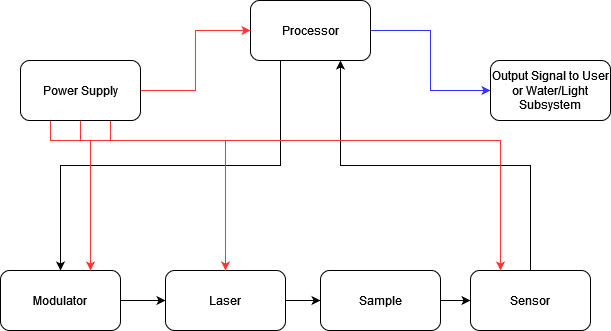
\includegraphics[width=\textwidth]{images/IRSensorBlockDiagram.png}
\end{figure}


The sensing subsystem is an infrared spectrometer that uses two photodiodes as detectors, a diffraction grating as a spectral separator, an array of LEDs to illuminate the target area, and optics to collect, collimate, and focus the beam.


\begin{figure}[H]
    \caption{Diffraction angle calculation}
    \centering
    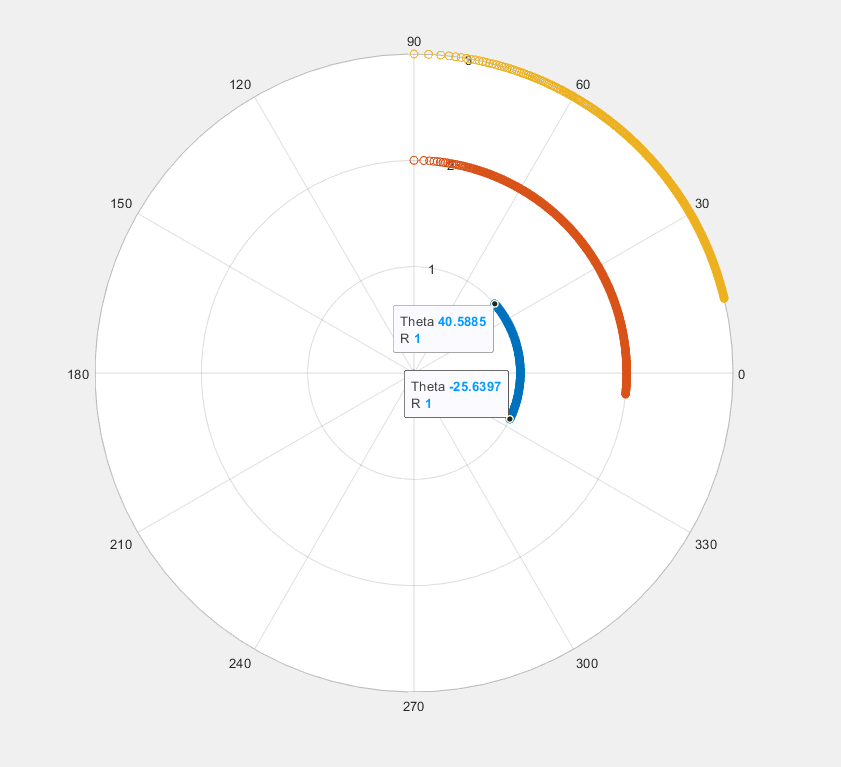
\includegraphics[width=\textwidth]{images/DiffractionAngleCalculator.png}
\end{figure}

\begin{figure}[H]
    \caption{Photodiode Signal Filter}
    \centering
    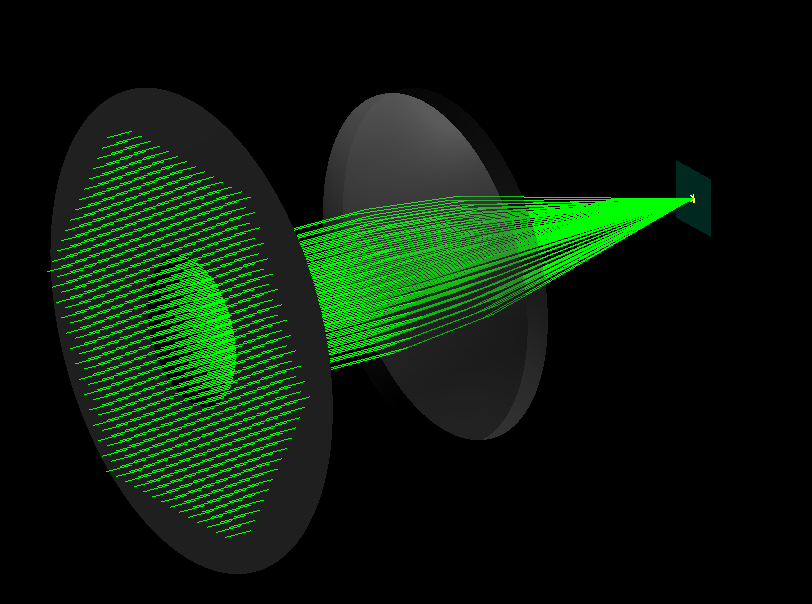
\includegraphics[width=\textwidth]{images/ColimatedBeam.png}
\end{figure}


\begin{figure}[H]
    \caption{Photodiode Signal Filter}
    \centering
    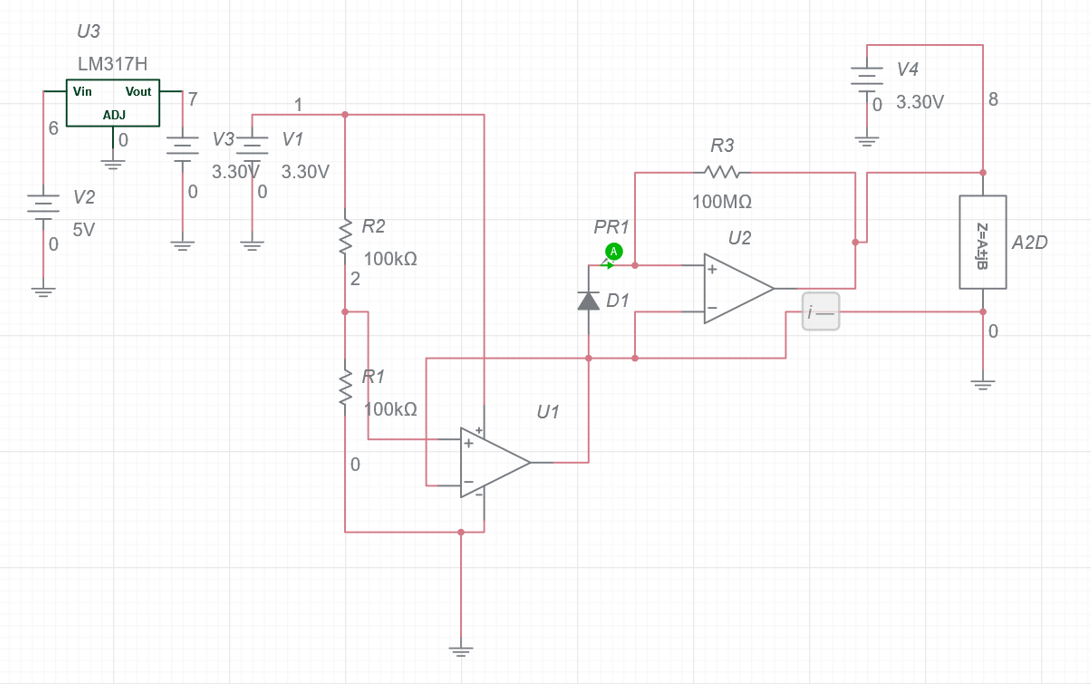
\includegraphics[width=\textwidth]{images/ElectricalSignalFilteringSD1.png}
\end{figure}


The Photodiode works by converting a small portion of the incident light into electrical current across the face of the semiconductor. The diode will have a small current running through the circuit hooked up to an amplifier for boosting the signal to a detectable level. Then another op amp will cut out the electrical noise created by unwanted frequencies generated by the diode and electromagnetic interference.

